\section{Условие}

Необходимо изучить и реализовать генератор псевдослучаных чисел программным и табличным методом. Получить 1, 2 и 3-хразрядные числа. Сравнить по критерию, сделать выводы.

\section{Генераторы}

В данной лабораторной рассматриваются табличный и программный методы генерирования псевдослучайных чисел. \textbf{Табличный генератор} -- это генератор, использующий таблицу некоррелированных цифр, то есть цифр, которые никак не зависят друг от друга. \textbf{Программный генератор} -- это генератор, формирующий псевдослучайные числа с помощью последовательности, в которой каждое сгенерированное число зависит от предыдущего.

\section{Критерии случайности}

\subsection{Частотный критерий}

Частотный критерий позволяет определить равномерность сгенерированных чисел блогодаря количеству чисел в интервале $(\mu - \sigma; \mu + \sigma)$, где $\mu$ -- математическое ожидание равномерной случайной величины, а $\sigma$ -- среднеквадратичное отклонение. Для ожидаемого (идеального) результата возьмем отношение длины рассматриваемого интервала к длине всего промежутка, на котором генерируется последовательность. Сравнивать с ожидаемым результатом будем отношение количества сгенерированных чисел на интервале к количеству всех сгенерированных чисел.

\subsection{$\chi^2$ критерий}

Принцип $\chi^2$ критерия заключается в нескольких шагах:

\begin{enumerate}
    \item вся последовательность делится на $k$ равных интевалов;
    \item определяется количество $n_i$ чисел, попавших в каждый интервал, при этом $n_1 + n_2 + \ldots + n_k = N$, где $N$ -- количество сгенерированных чисел;
    \item вычисляется экспериментальное значение $\chi^2_\text{эксп}$ по формуле \ref{eq:chi}

        \begin{equation}\label{eq:chi}
            \chi^2_\text{эксп} = \frac{1}{N} \sum_{i=1}^k \bigg( \frac{n_i^2}{p_i} \bigg) - N,
        \end{equation}

        где $p_i = \frac{1}{k}$ -- теоретическая вероятность попадания чисел в $k$-ый интервал;

    \item затем $\chi^2_\text{эксп}$ сравнивается с теоретической величиной $\chi^2_\text{теор}$, взятой из таблицы значений, откуда находится параметр $p$ -- вероятность того, что экспериментальное значение критерия $\chi^2$ будет меньше или равно теоретического.
\end{enumerate}

\section{Полученные результаты}

\begin{figure}[H]
    \centering
    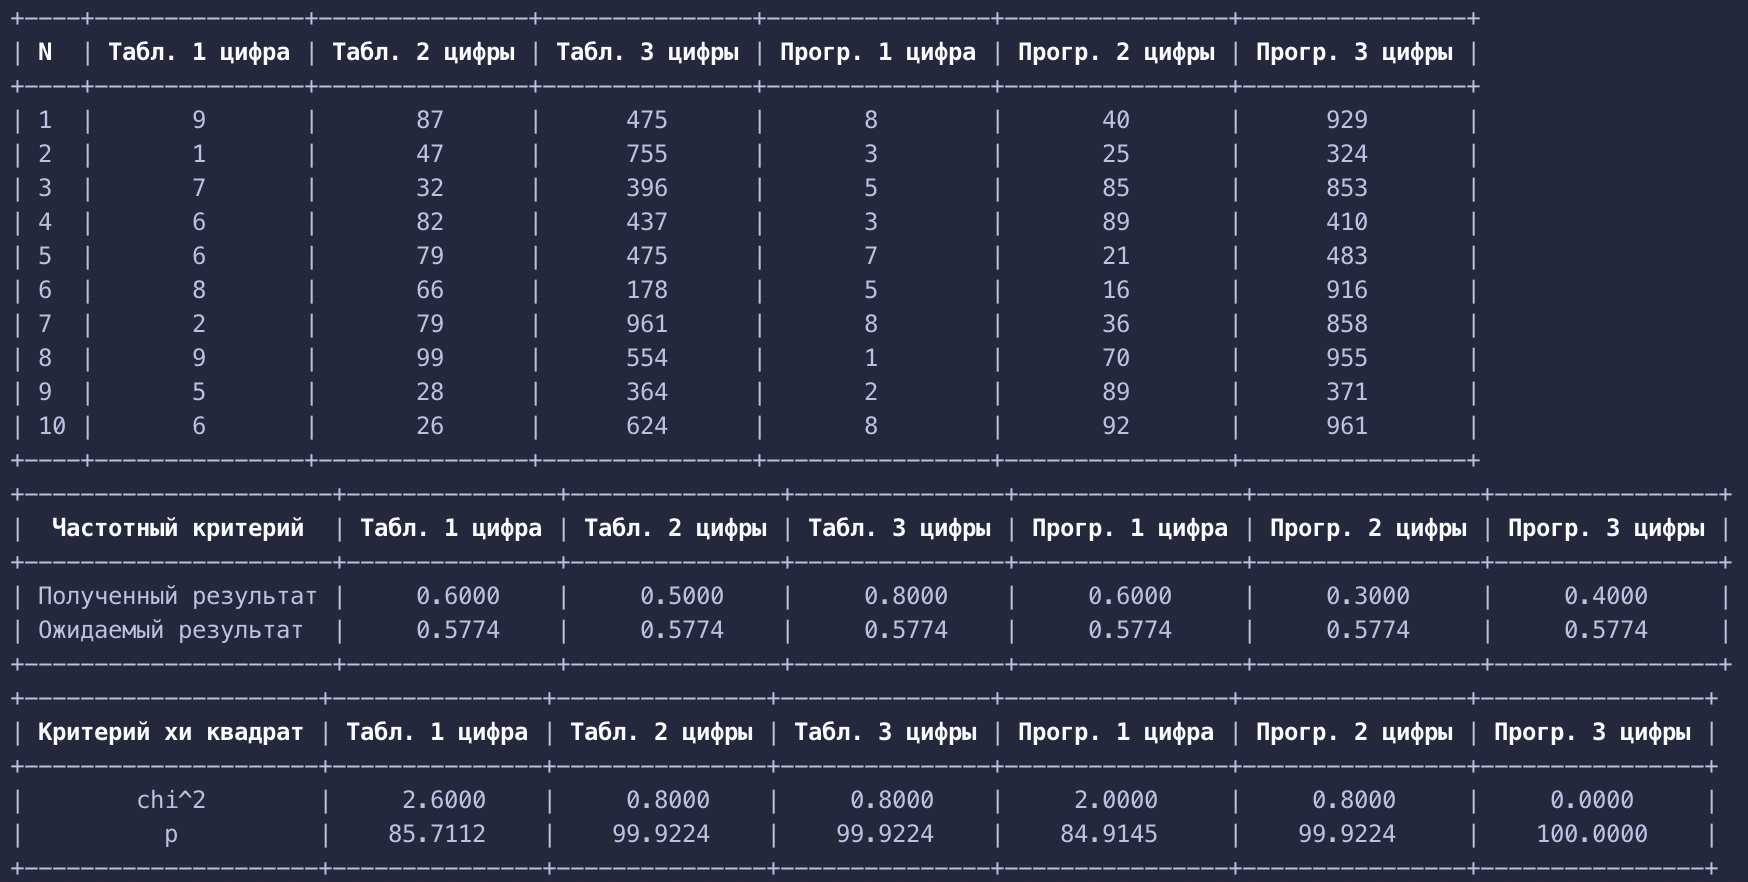
\includegraphics[width=0.8\textwidth]{img/content/10.png}
    \caption{Результаты для 10 чисел}
    \label{fig:}
\end{figure}

\begin{figure}[H]
    \centering
    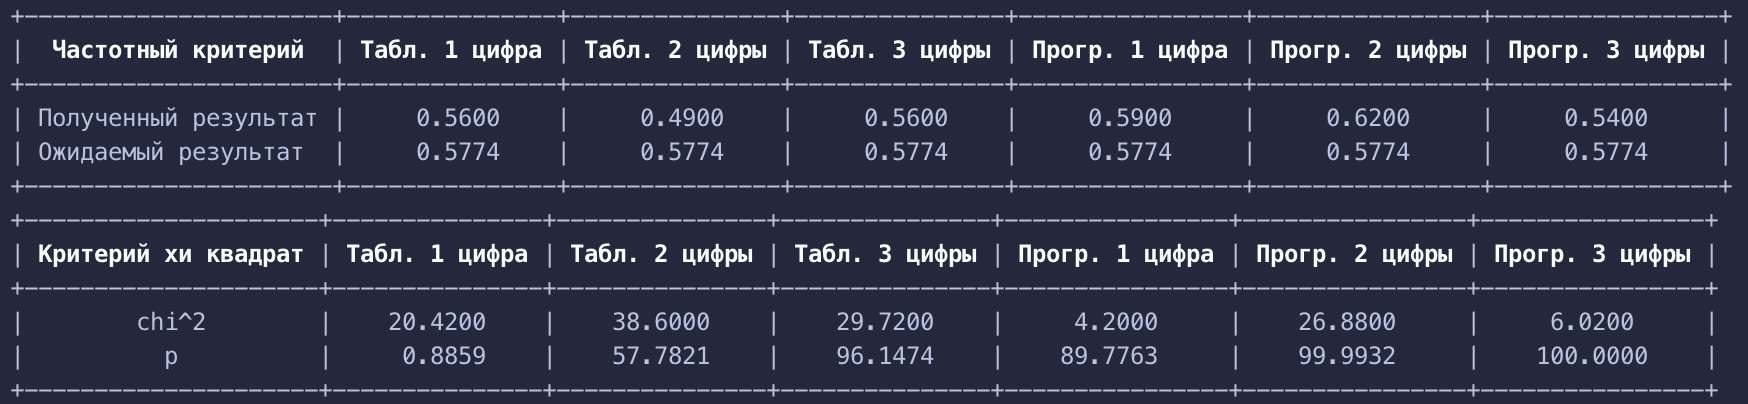
\includegraphics[width=0.8\textwidth]{img/content/100.png}
    \caption{Результаты для 100 чисел}
    \label{fig:}
\end{figure}

\begin{figure}[H]
    \centering
    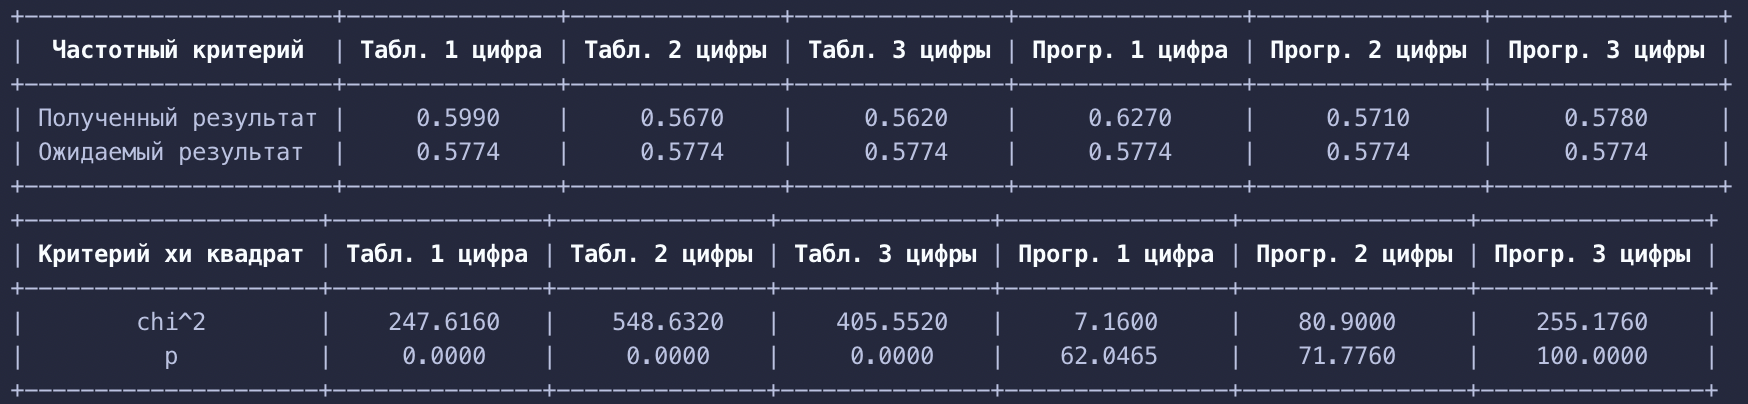
\includegraphics[width=0.8\textwidth]{img/content/1000.png}
    \caption{Результаты для 1000 чисел}
    \label{fig:}
\end{figure}

\section{Вывод}

Выполнив данную лабораторную работу можно сделать вывод о том, что чем больше количество генерируемых чисел, тем более равномерно они распределены. Так же можно заметить по полученным результатам, что программный метод работает лучше, чем табличный.
